% Created 2026-04-23 Thu 12:08
% Intended LaTeX compiler: lualatex
\DocumentMetadata{lang = en-US,pdfversion = 2.0,pdfstandard = ua-2,tagging = on,tagging-setup = {math/setup=mathml-SE},}
\documentclass[11pt]{article}
\usepackage{amsmath}
\usepackage{fontspec}
\usepackage{graphicx}
\usepackage{longtable}
\usepackage{wrapfig}
\usepackage{rotating}
\usepackage[normalem]{ulem}
\usepackage{capt-of}
\usepackage{hyperref}
\usepackage[margin=1in]{geometry}
\usepackage{fontspec}
\usepackage{verbatim, multicol, tabularx,}
\usepackage{amsmath, amsthm, amssymb, stmaryrd, latexsym, bm, listings, qtree}
\usepackage{framed}
\usepackage{xcolor,colortbl}
\usepackage{media9}
\usepackage[export]{adjustbox}
\usepackage{algorithm}
\usepackage[noend]{algpseudocode}
\usepackage{tikz,pgfplots}
\usetikzlibrary{shapes.geometric}
\let\oldquote=\quote
\let\endoldquote=\endquote
\colorlet{shadecolor}{cyan!15}
\renewenvironment{quote}{\begin{shaded*}\begin{oldquote}}{\end{oldquote}\end{shaded*}}
% From https://tex.stackexchange.com/questions/7032/good-way-to-make-textcircled-numbers
\newcommand*\circled[1]{\tikz[baseline=(char.base)]{\node[shape=circle,draw,inner sep=2pt] (char) {#1};}}
\DeclareMathOperator*{\argmin}{arg\!min}
\DeclareMathOperator*{\argmax}{arg\!max}
\lstset{frame=tb, aboveskip=1mm, belowskip=0mm, showstringspaces=false, columns=flexible, basicstyle={\scriptsize\ttfamily}, numbers=left, frame=single, breaklines=true, breakatwhitespace=true}
\hypersetup{colorlinks=true,urlcolor=blue}
\usepackage{tagpdf}
\tagpdfsetup{activate-all}
\tagpdfsetup{math/alt/use}
\usepackage{polyglossia}
\setdefaultlanguage[variant=en-US]{english}
\author{Christopher Simpkins}
\date{Kennesaw State University}
\title{Artificial Intelligence\\\medskip
\large Inference in First-Order Logic}
\hypersetup{
 pdfauthor={Christopher Simpkins},
 pdftitle={Artificial Intelligence},
 pdfkeywords={},
 pdfsubject={Artificial Intelligence Inference in First-Order Logic},
 pdfcreator={Emacs 30.2 (Org mode 9.7.11)}, 
 pdflang={English}}
\begin{document}

\maketitle
\section{Propositional vs. First-Order Logc}
\label{sec:orga57e20a}

Foo
\section{Unification and First-Order Inference}
\label{sec:org900fe82}


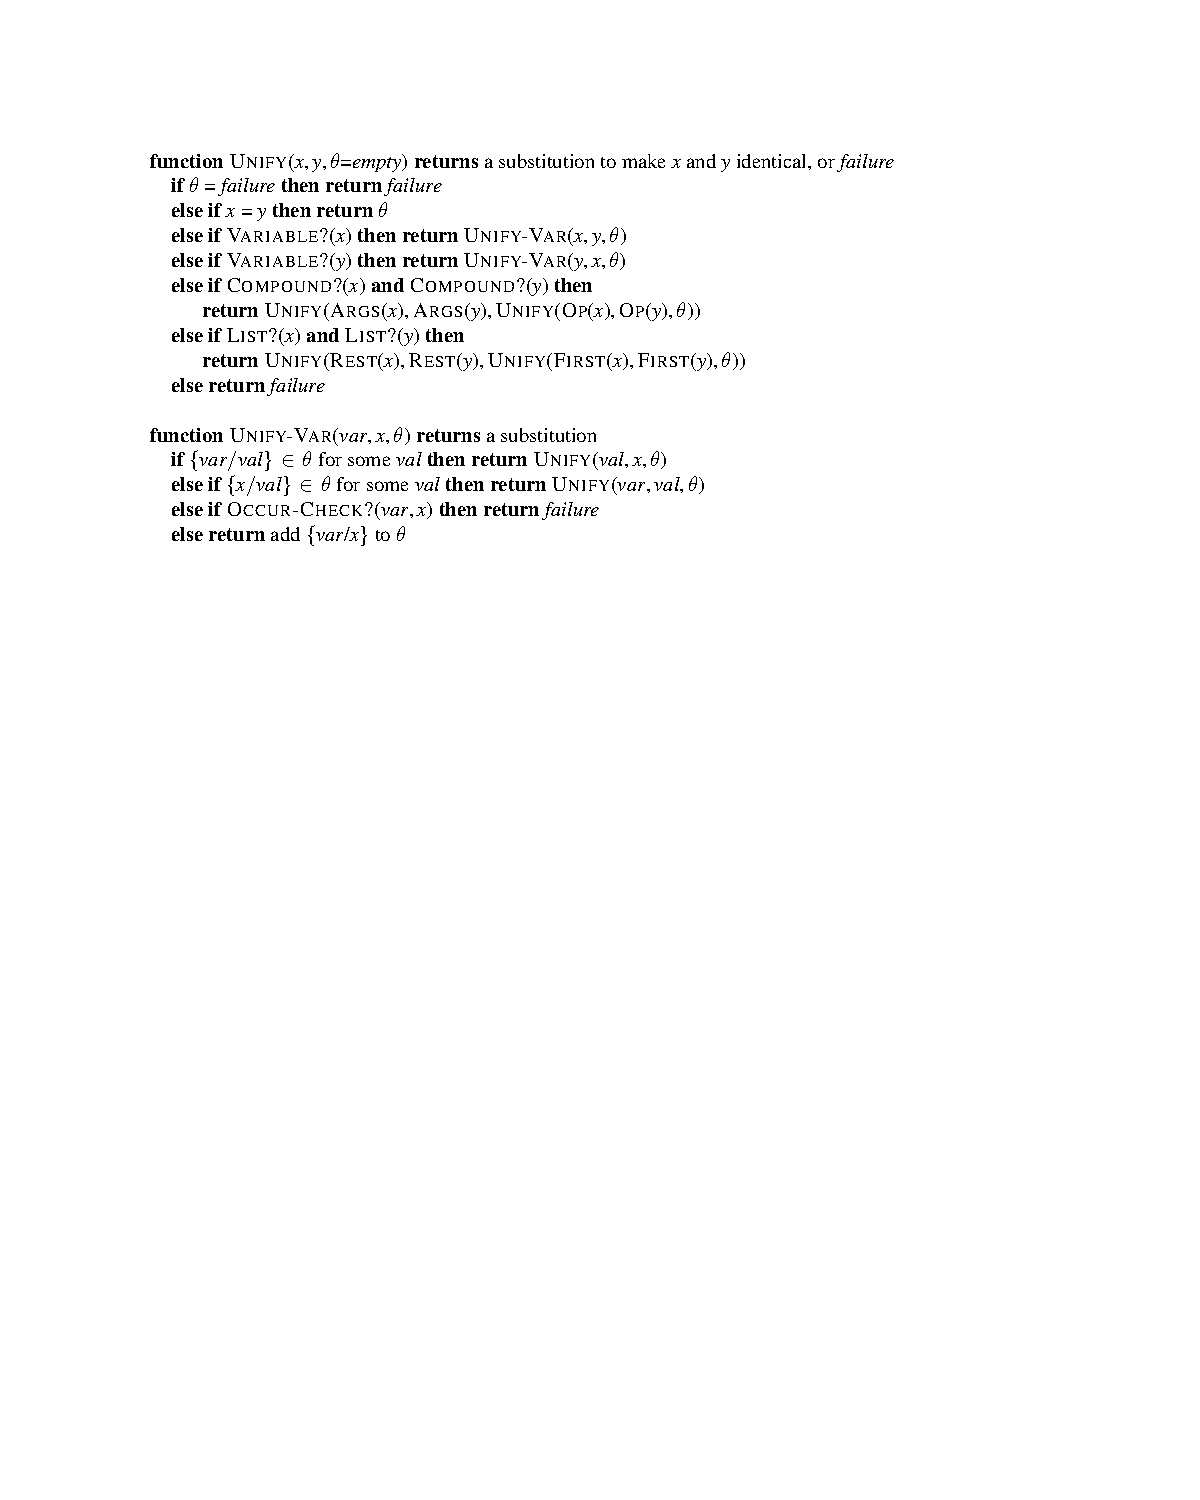
\includegraphics[alt={aima fig 09_01 unification algorithm},height=2.8in]{aima-fig-09_01-unification-algorithm.pdf}
\section{Unification and First-Order Inference}
\label{sec:orgfbcd2c8}


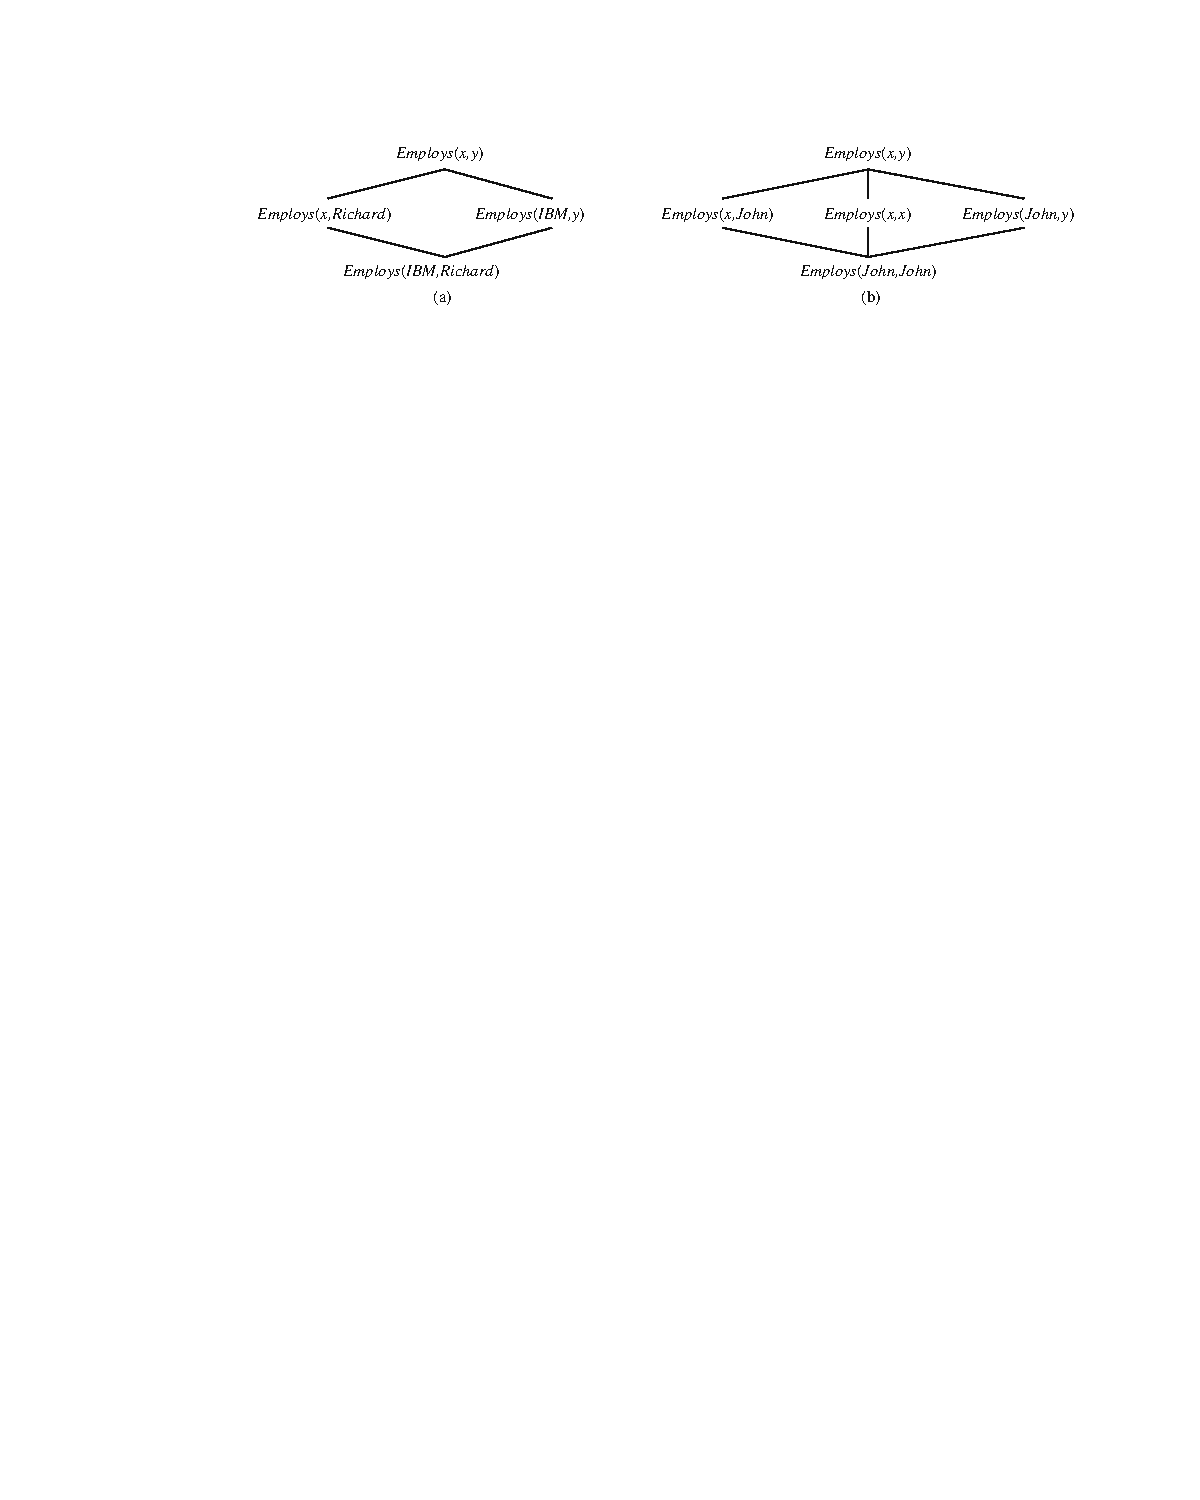
\includegraphics[alt={aima fig 09_02 subsumption lattice},height=2.8in]{aima-fig-09_02-subsumption-lattice.pdf}
\section{Forward Chaining}
\label{sec:orgef39d98}


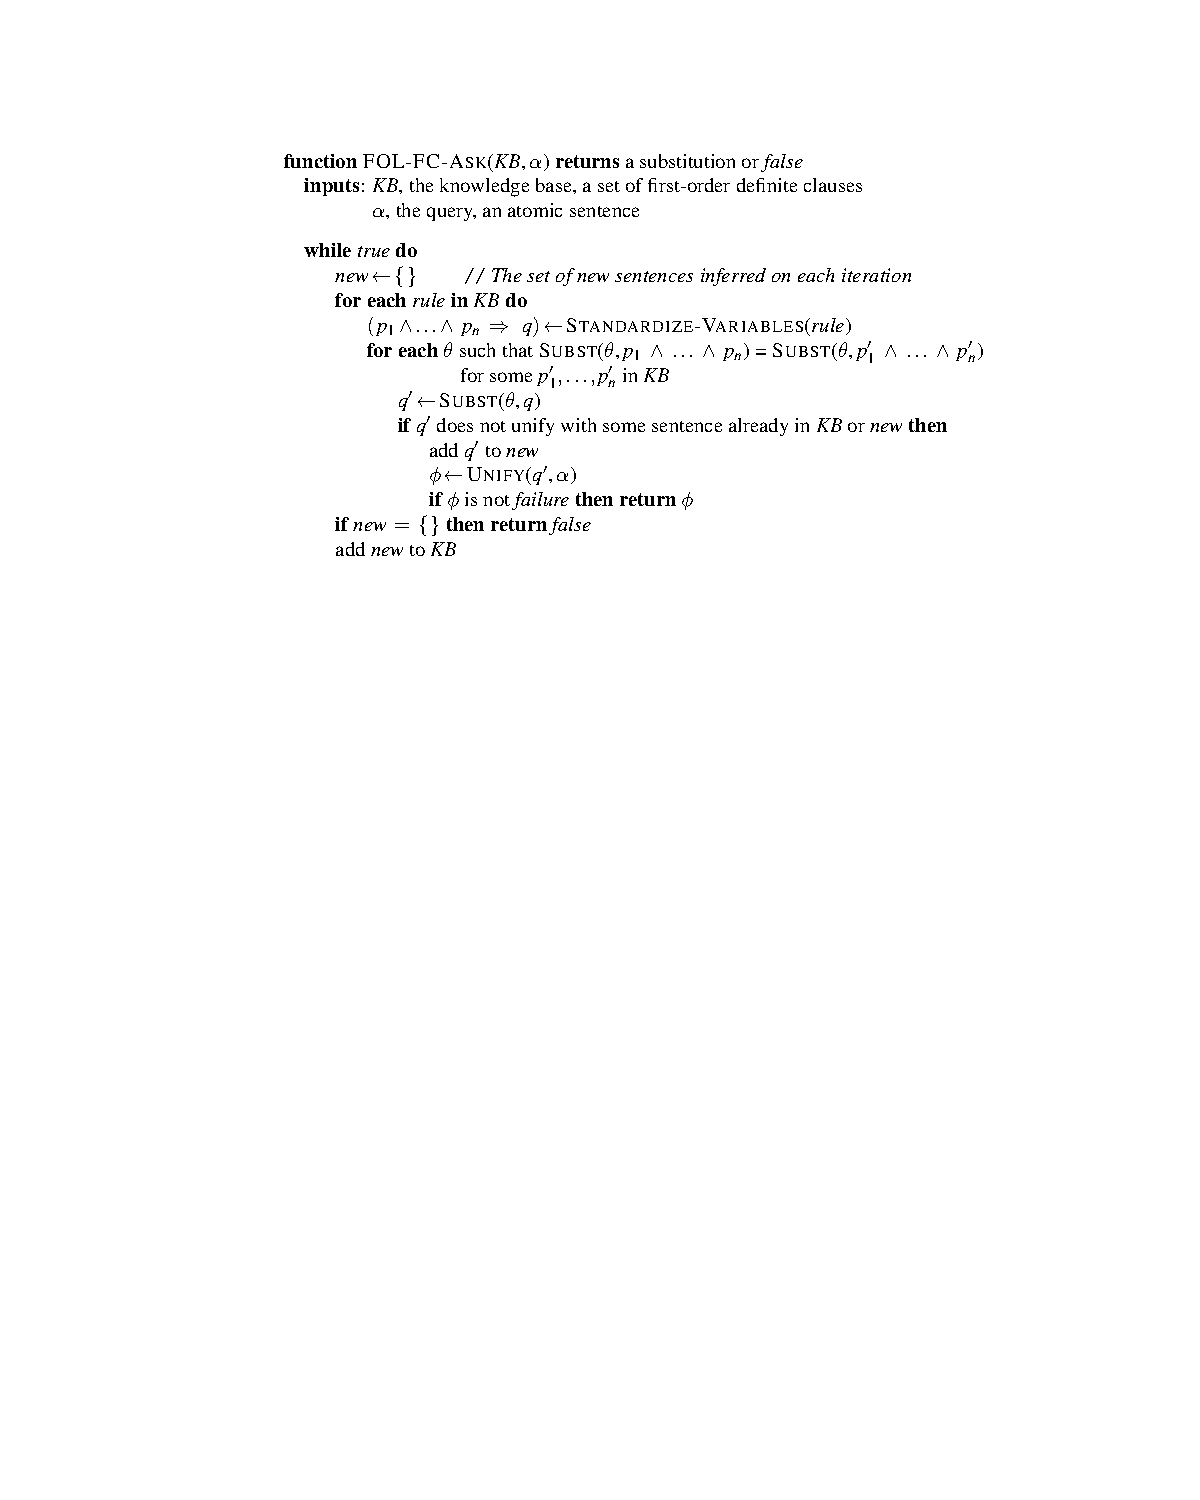
\includegraphics[alt={aima fig 09_03 fol fc ask algorithm},height=2.8in]{aima-fig-09_03-fol-fc-ask-algorithm.pdf}
\section{Forward Chaining}
\label{sec:org15d9fac}


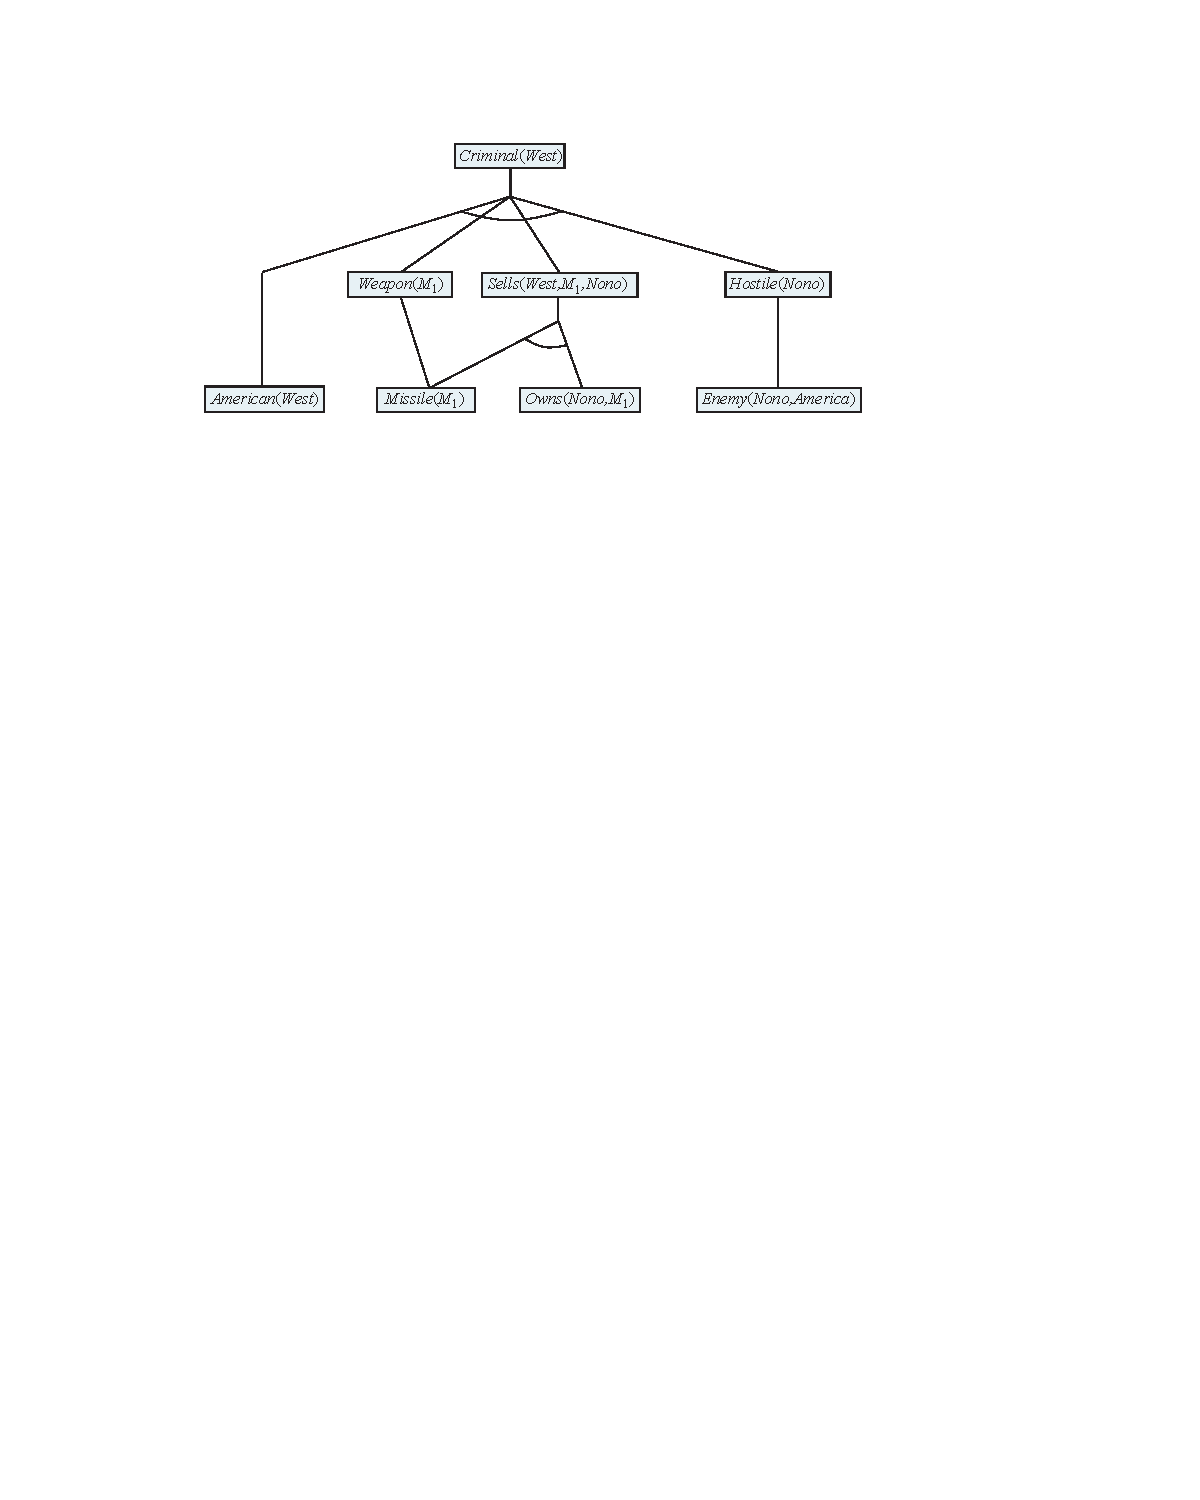
\includegraphics[alt={aima fig 09_04 proof tree fc crime},height=2.8in]{aima-fig-09_04-proof-tree-fc-crime.pdf}
\section{Forward Chaining}
\label{sec:orgf3241cc}


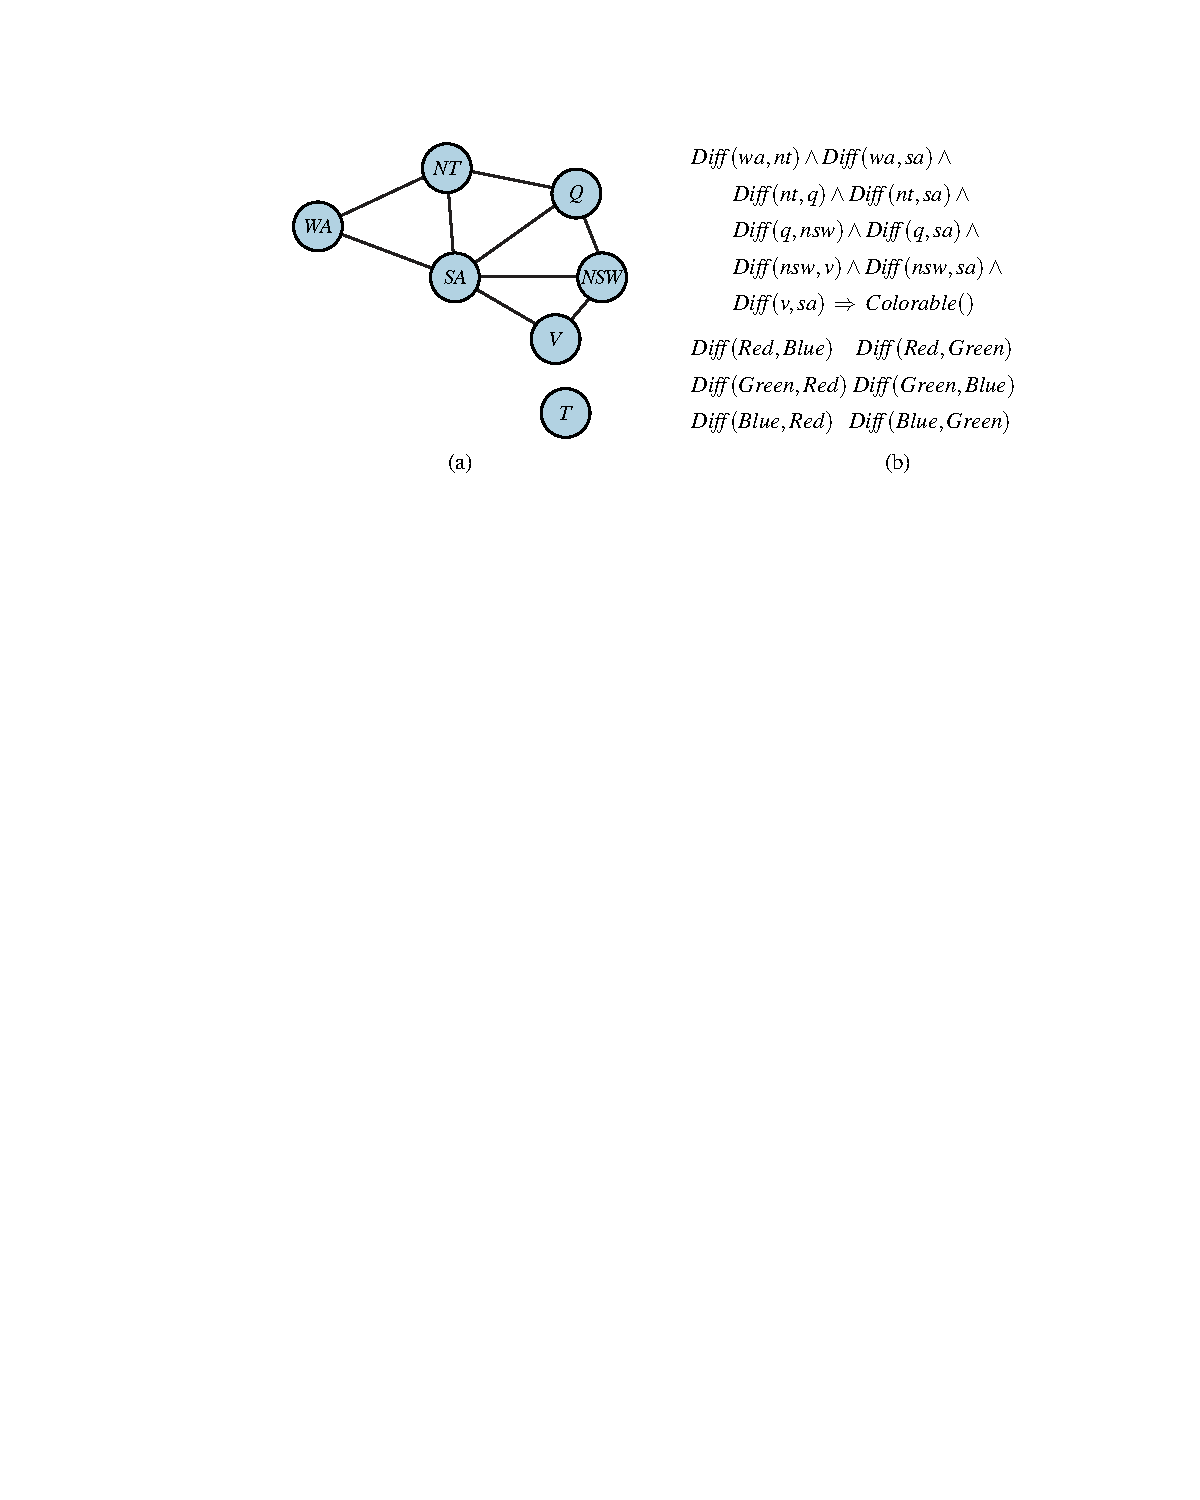
\includegraphics[alt={aima fig 09_05 constraint graph australia},height=2.8in]{aima-fig-09_05-constraint-graph-australia.pdf}
\section{Backward Chaining}
\label{sec:org94841e1}


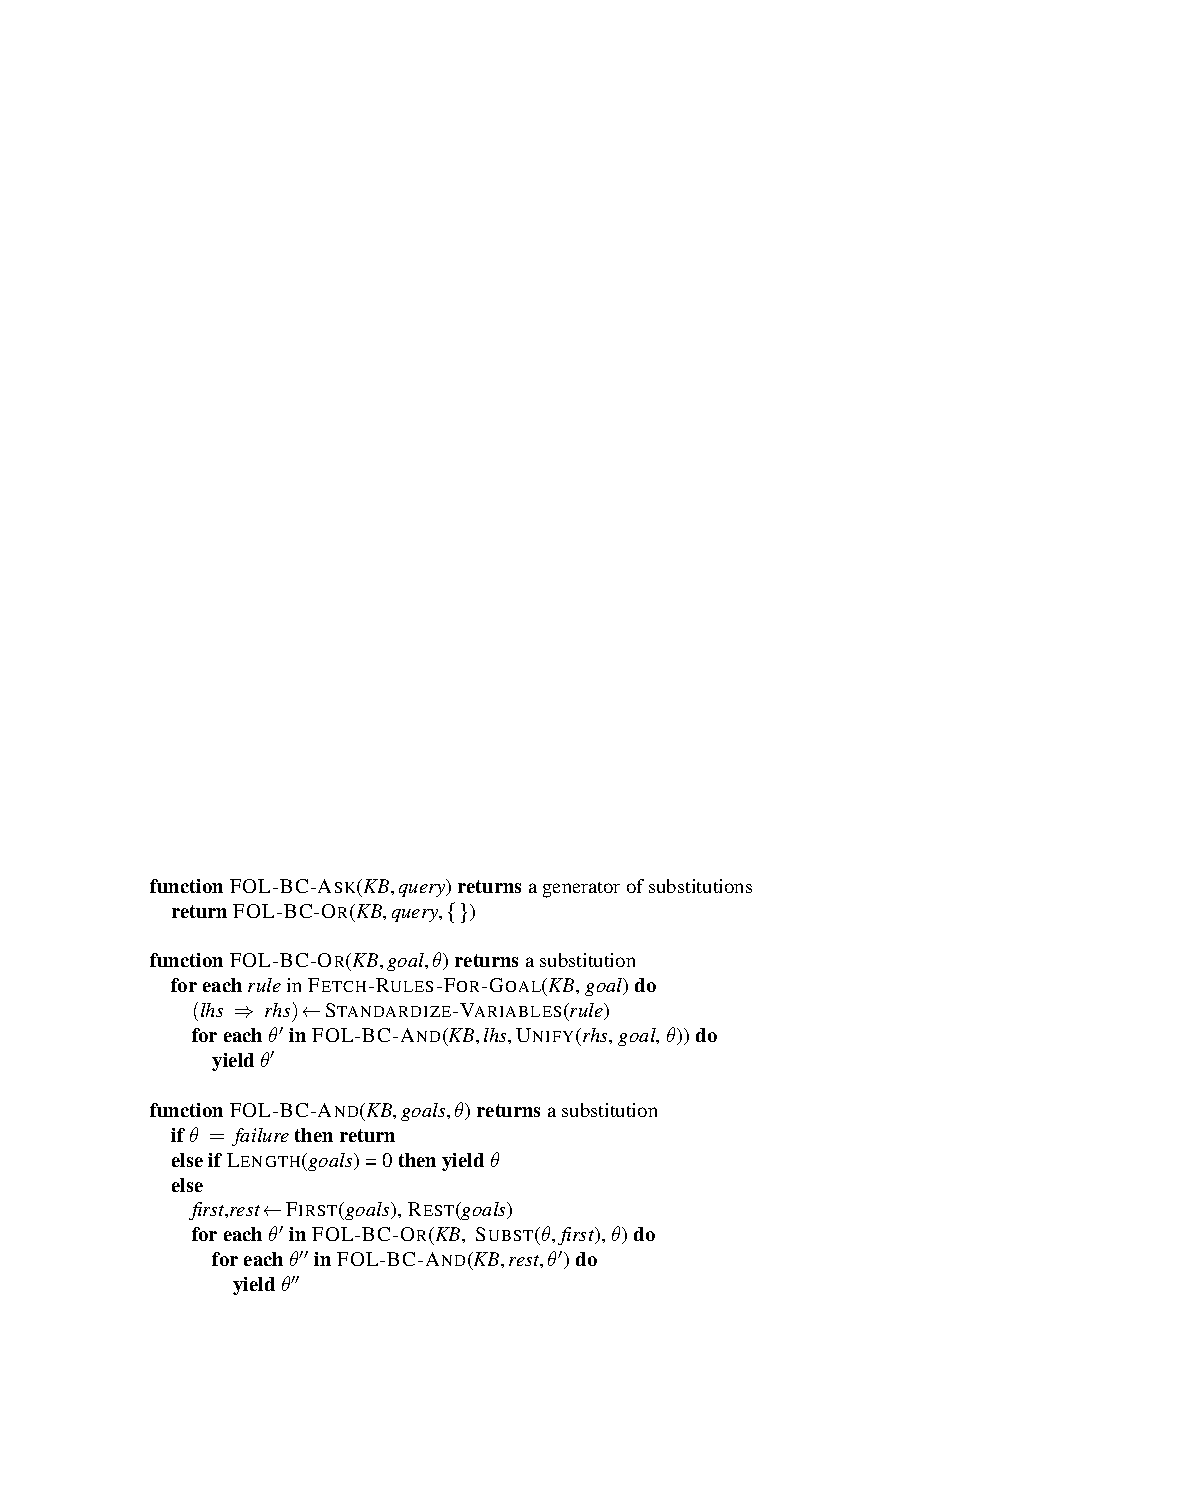
\includegraphics[alt={aima fig 09_06 fol bc ask algorithm},height=2.8in]{aima-fig-09_06-fol-bc-ask-algorithm.pdf}
\section{Backward Chaining}
\label{sec:org56a5546}


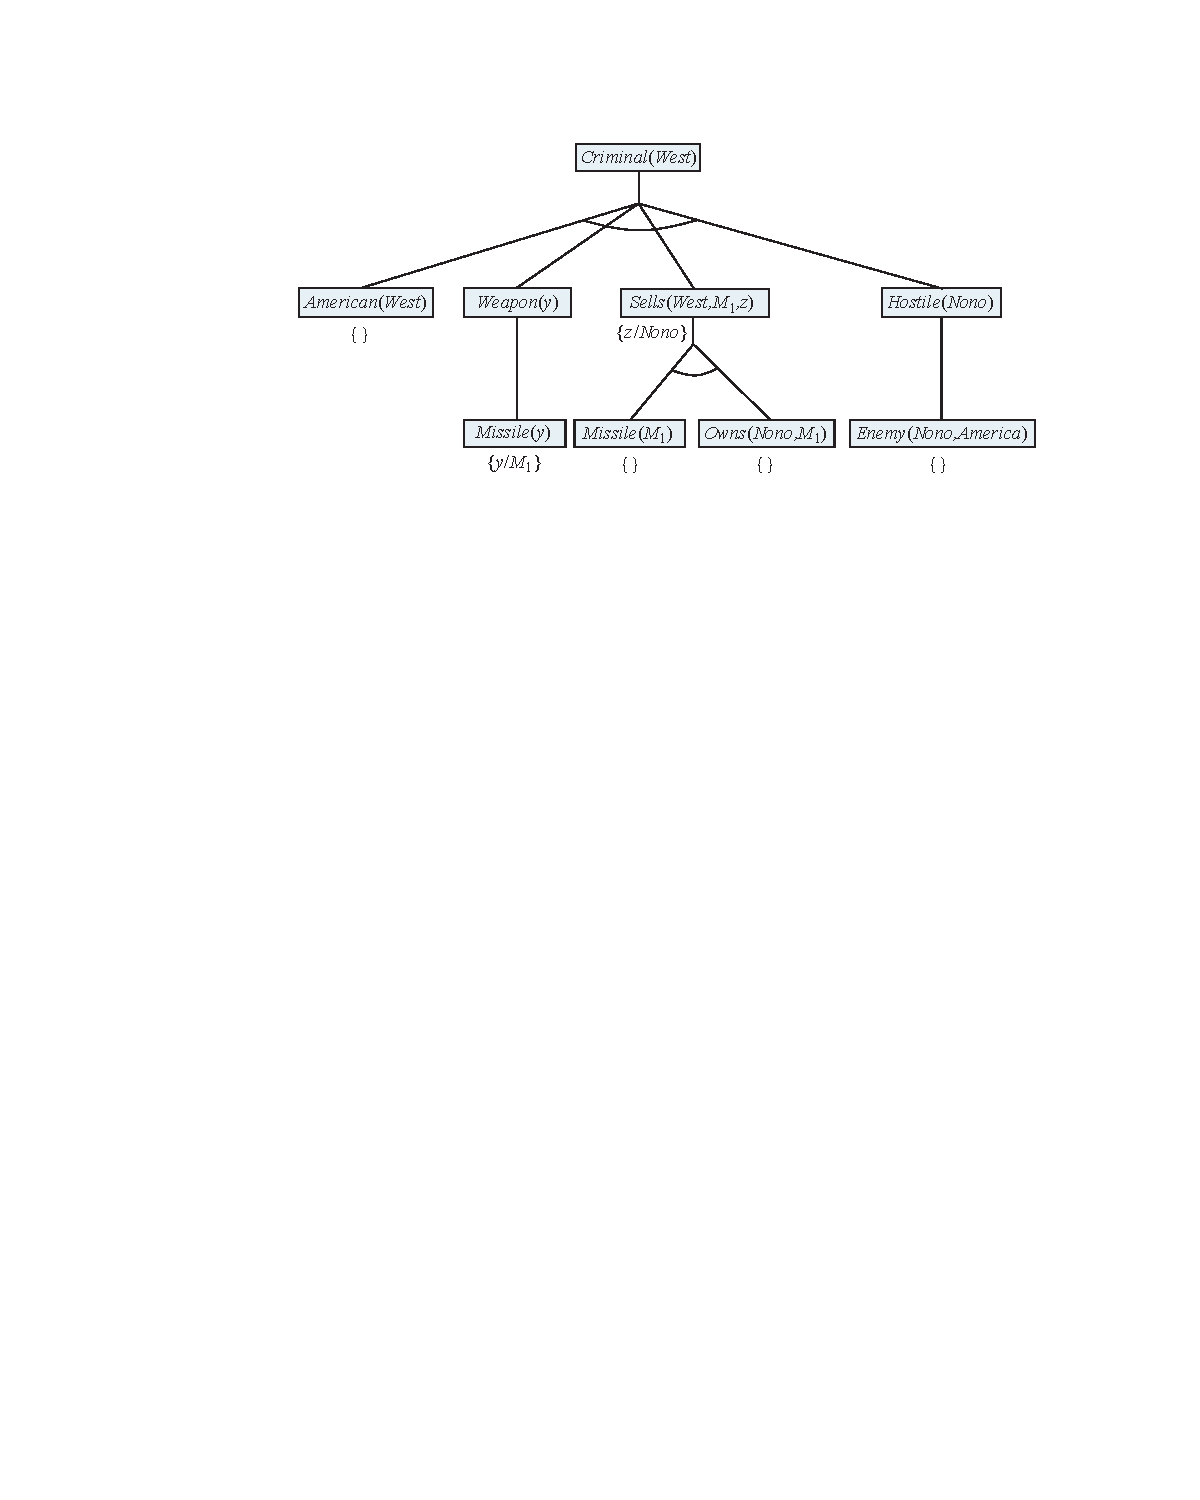
\includegraphics[alt={aima fig 09_07 proof tree bc crime},height=2.8in]{aima-fig-09_07-proof-tree-bc-crime.pdf}
\section{Logic Programming}
\label{sec:orgfe9859d}


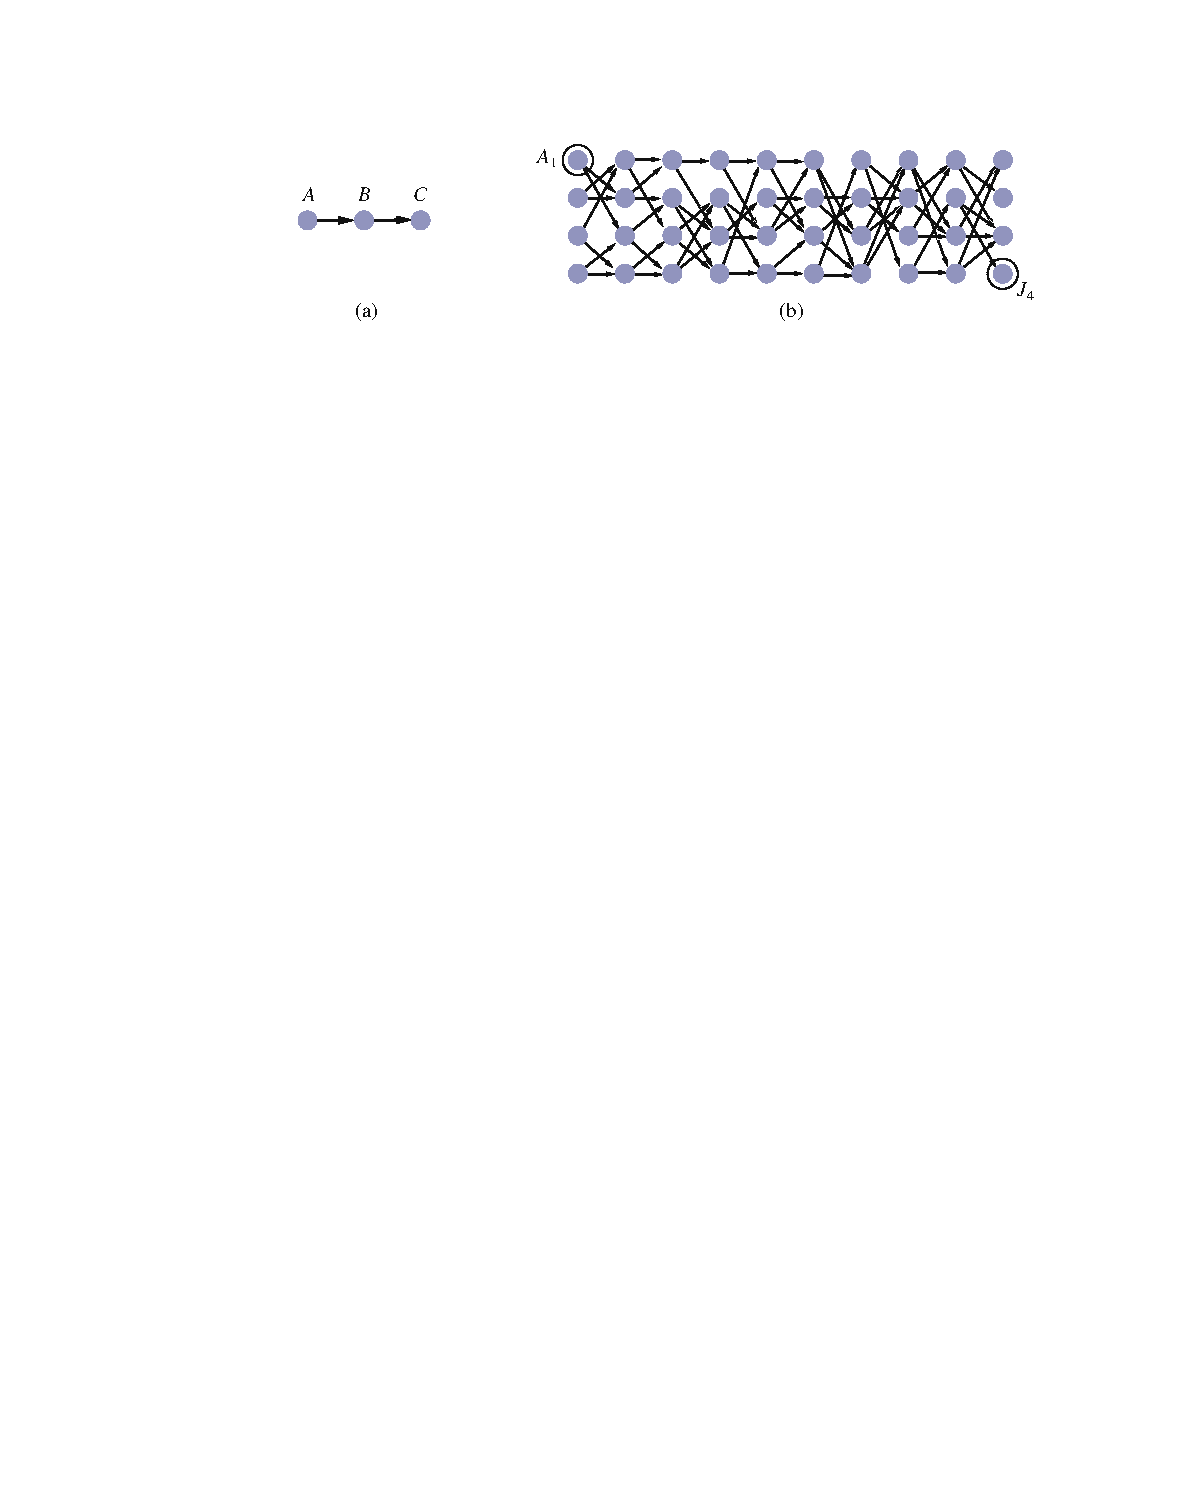
\includegraphics[alt={aima fig 09_08 prolog infinite loop},height=2.8in]{aima-fig-09_08-prolog-infinite-loop.pdf}
\section{Logic Programming}
\label{sec:orgcaa549f}


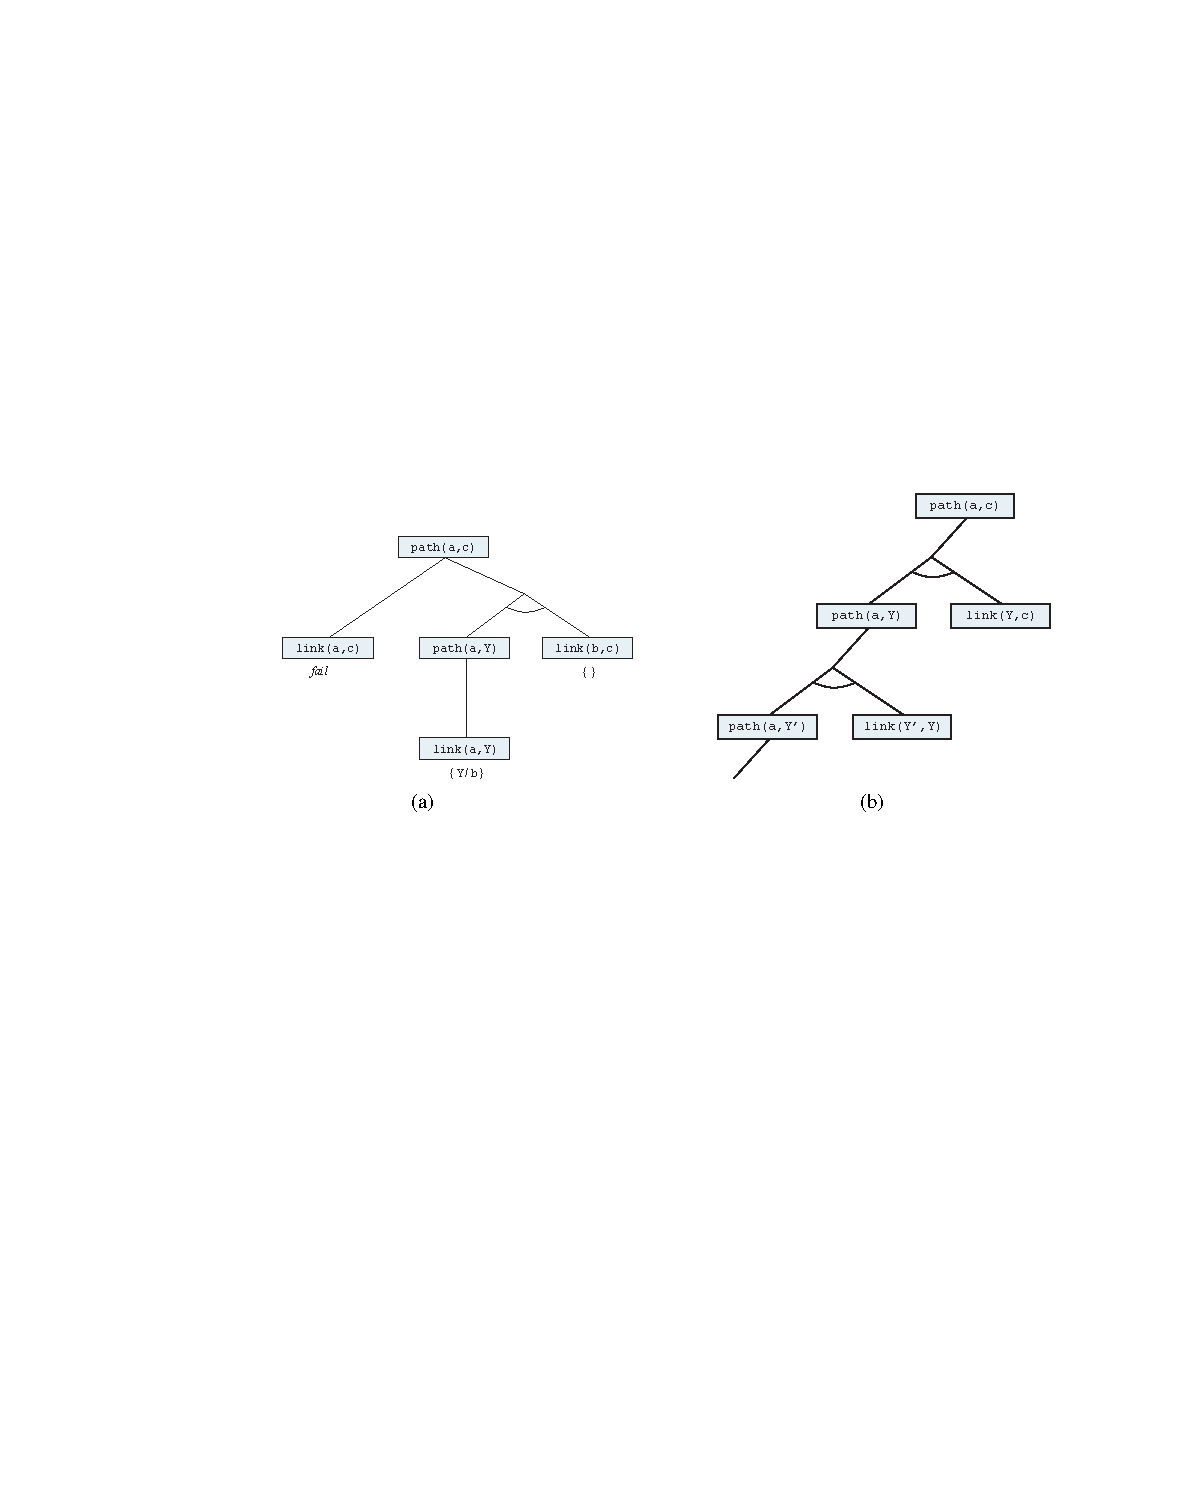
\includegraphics[alt={aima fig 09_09 infinite proof tree},height=2.8in]{aima-fig-09_09-infinite-proof-tree.pdf}
\section{Resolution}
\label{sec:orgdb8e761}


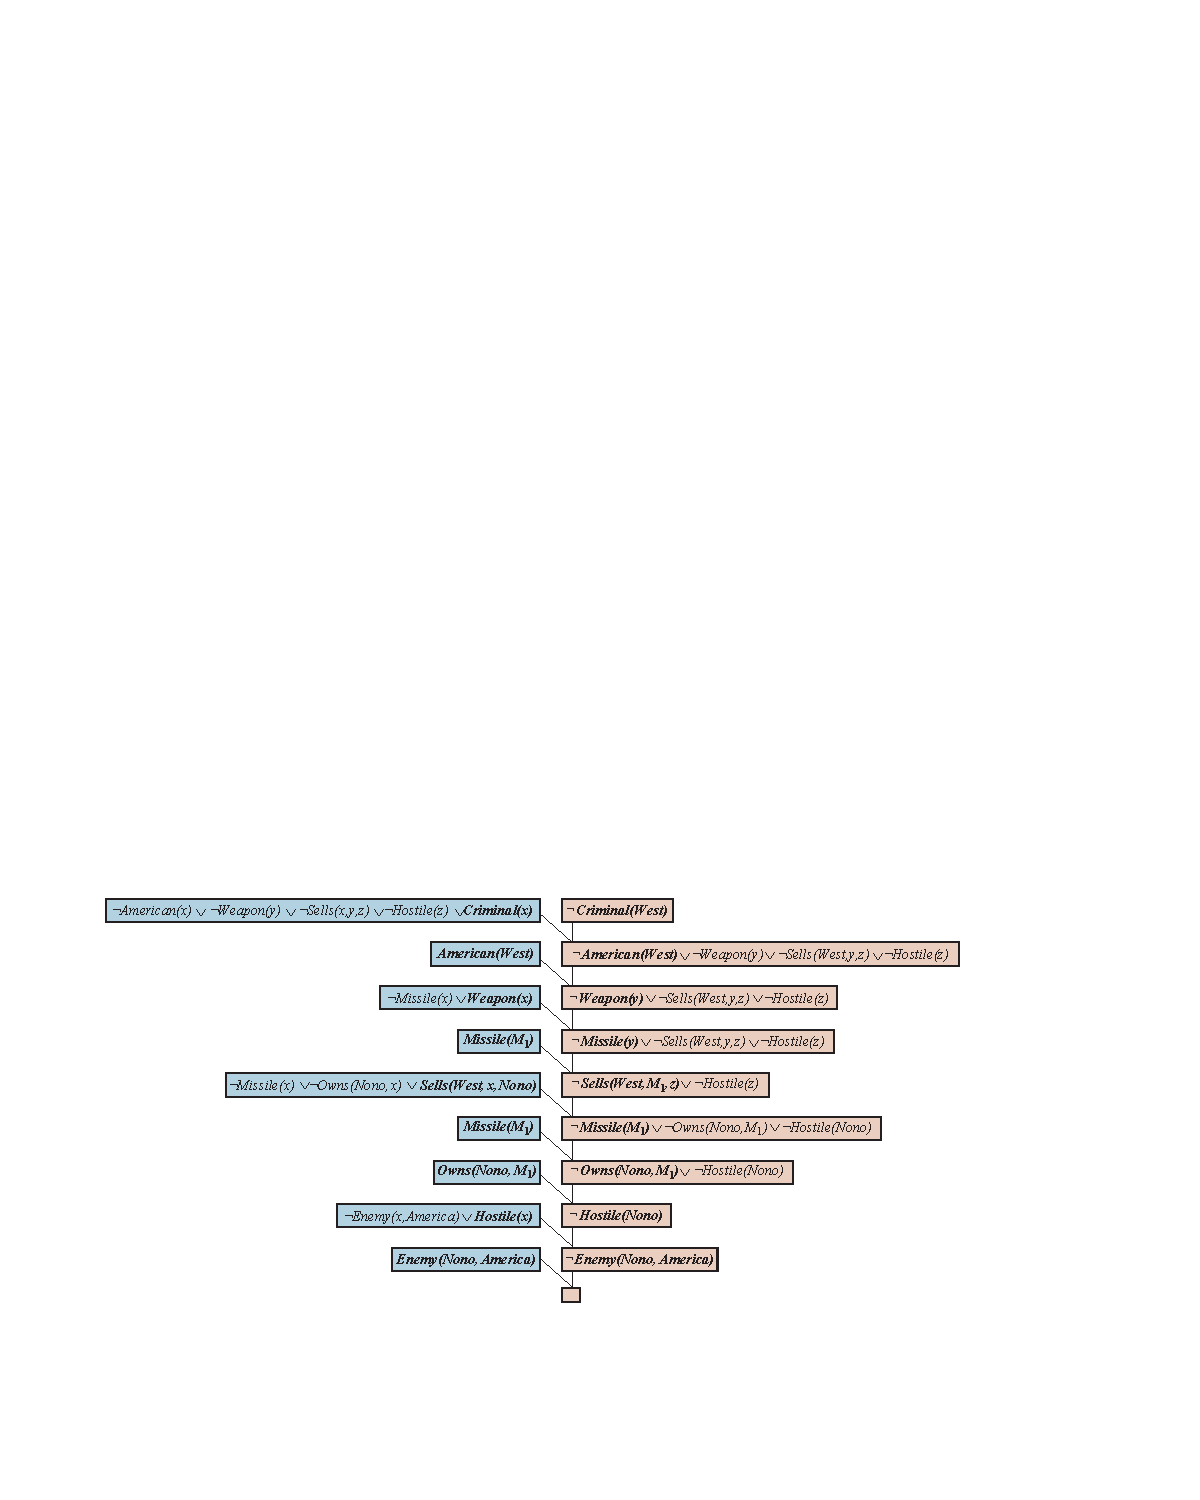
\includegraphics[alt={aima fig 09_10 resolution proof criminal},height=2.8in]{aima-fig-09_10-resolution-proof-criminal.pdf}
\section{Resolution}
\label{sec:org694f622}


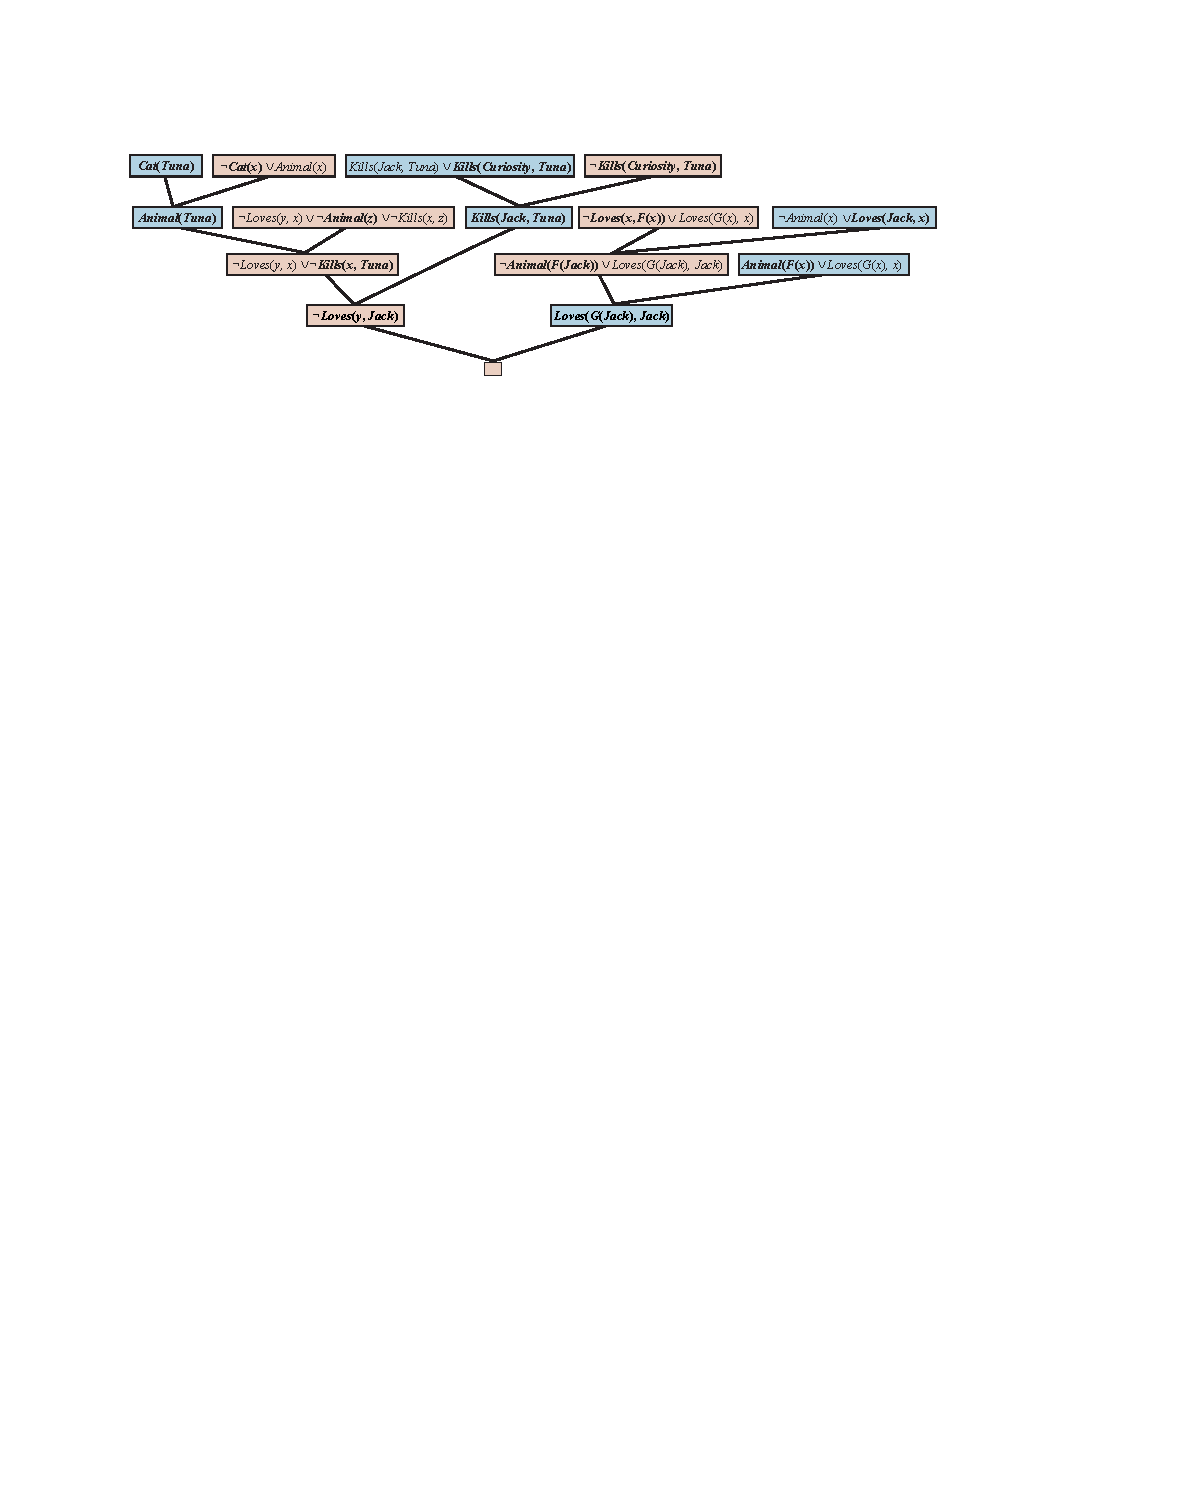
\includegraphics[alt={aima fig 09_11 resolution proof curiosity},height=2.8in]{aima-fig-09_11-resolution-proof-curiosity.pdf}
\section{Completeness}
\label{sec:orgae48849}


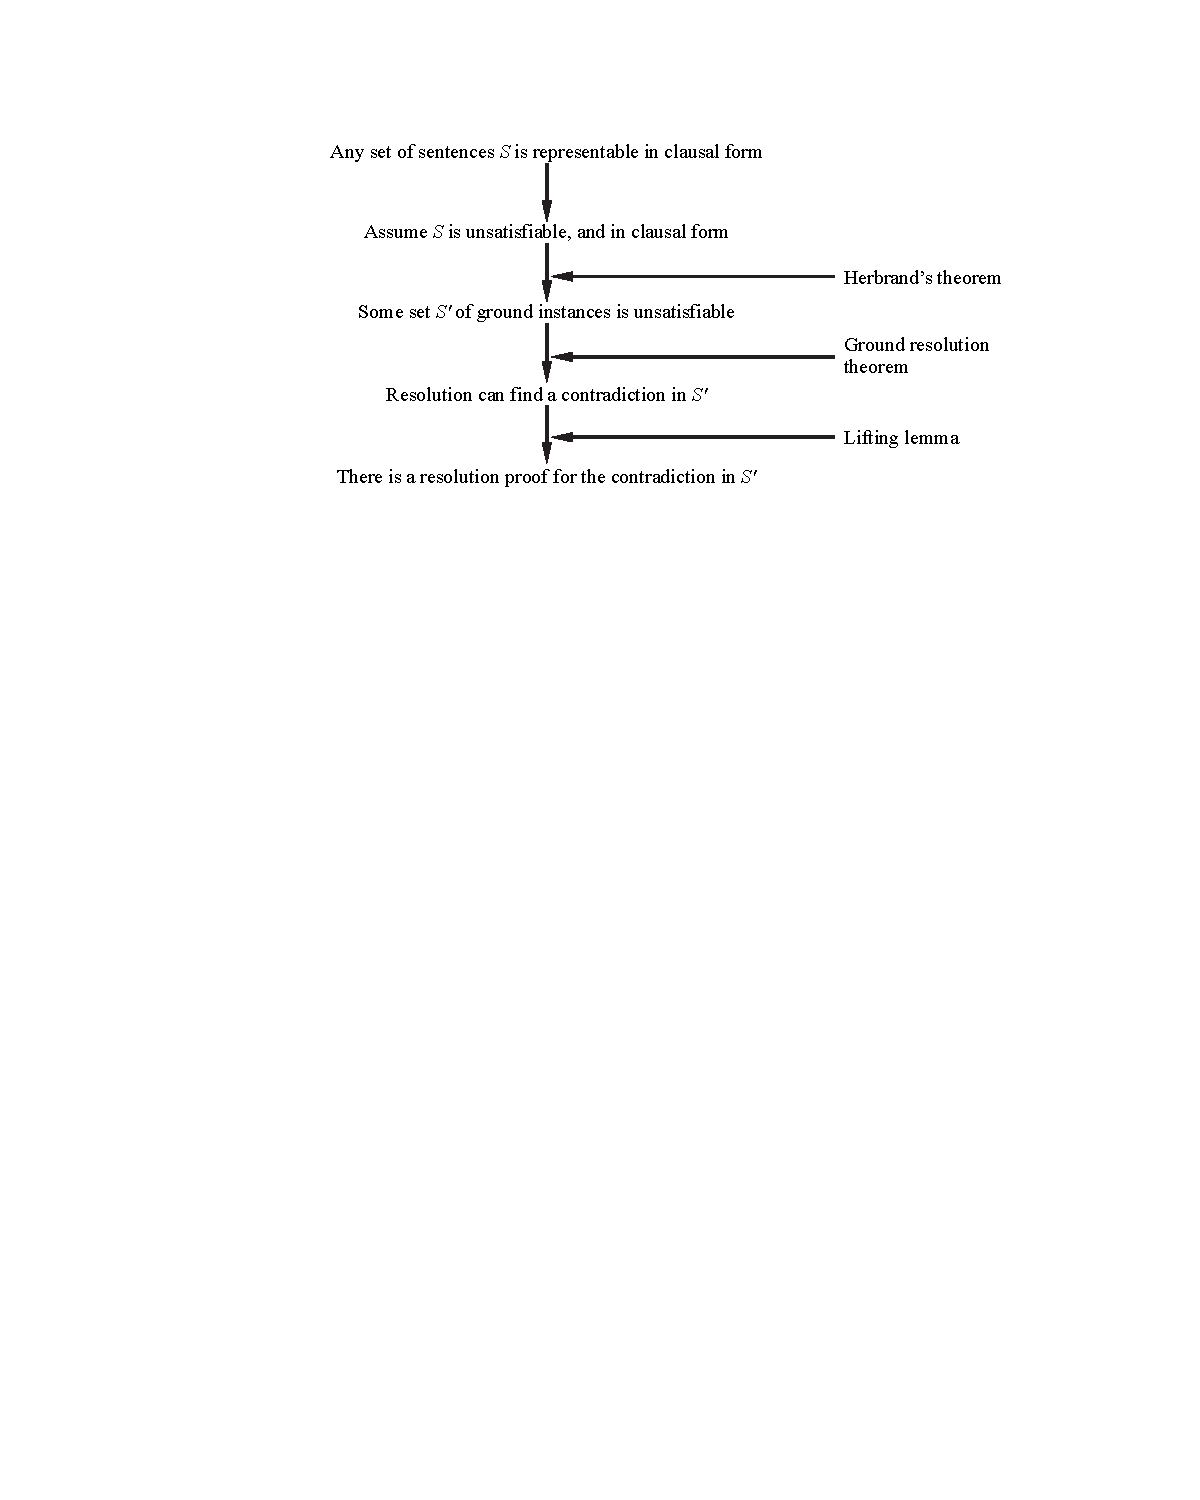
\includegraphics[alt={aima fig 09_12 structure completeness proof},height=2.8in]{aima-fig-09_12-structure-completeness-proof.pdf}
\section{G\{$\backslash$"o\}del's Incompleteness Theorem}
\label{sec:org8d3b259}

Foo
\end{document}
